\documentclass[10pt,twocolumn,letterpaper]{article}

\usepackage{cvpr}
\usepackage{times}
\usepackage{epsfig}
\usepackage{graphicx}
\usepackage{amsmath}
\usepackage{amssymb}

% Include other packages here, before hyperref.

% If you comment hyperref and then uncomment it, you should delete
% egpaper.aux before re-running latex.  (Or just hit 'q' on the first latex
% run, let it finish, and you should be clear).
\usepackage[breaklinks=true,bookmarks=false]{hyperref}

\cvprfinalcopy % *** Uncomment this line for the final submission

\def\cvprPaperID{****} % *** Enter the CVPR Paper ID here
\def\httilde{\mbox{\tt\raisebox{-.5ex}{\symbol{126}}}}

% Pages are numbered in submission mode, and unnumbered in camera-ready
%\ifcvprfinal\pagestyle{empty}\fi
\setcounter{page}{1}
\begin{document}

%%%%%%%%% TITLE
\title{Milestone: Understanding the Amazon from Space}

\author{Vishal Subbiah\\
Stanford University\\
{\tt\small svishal@stanford.edu}
% For a paper whose authors are all at the same institution,
% omit the following lines up until the closing ``}''.
% Additional authors and addresses can be added with ``\and'',
% just like the second author.
% To save space, use either the email address or home page, not both
\and
Brent Lunghino\\
Stanford University\\
{\tt\small lunghino@stanford.edu}
\and
Brian Rohr\\
Stanford University\\
{\tt\small brohr@stanford.edu}
}

\maketitle
%\thispagestyle{empty}

%%%%%%%%% ABSTRACT
\begin{abstract}
   In this work, we use convolutional neural networks to assign atmospheric conditions labels and land usage labels to satellite images of the Amazon Rainforest. We have trained several neural networks and submitted results to the Kaggle.com competition. To date, our best result is 0.83 (F2 score) on the validation set, but we expect to be able to improve on that result going forward by using data augmentation, deeper architectures, and more fine-tuned hyperparameter optimization.
\end{abstract}

%%%%%%%%% BODY TEXT]

\iffalse
\section{GUIDELINES}

\begin{itemize}
\item Your project milestone report should be between 2 - 3 pages using the provided template. The following is a suggested structure for your report:\newline
\item Title, Author(s)\newline
\item Introduction: this section introduces your problem, and the overall plan for approaching your problem\newline
\item Problem statement: Describe your problem precisely specifying the dataset to be used, expected results and evaluation\newline
\item Technical Approach: Describe the methods you intend to apply to solve the given problem\newline
\item Intermediate/Preliminary Results: State and evaluate your results upto the milestone
\item Submission: Please upload a PDF file to the assignments tab on Canvas. Please have one person on your team submit your milestone. If you submit your milestone late, all team members will be charged late days.
\end{itemize}

\fi

\section{Introduction}

	The Amazon Rainforest is extremely important to preserve due to its unmatched biodversity and great capacity to uptake carbon dioxide \cite{WWF}, but it is difficult to make a case for the urgency of its preservation without first quantifying the rate of its destruction.  Since the Amazon covers a 5.5 million square kilometer area, understanding and quantifying the changes in land use there over the years is a formidable task. With a great deal of effort, humans could classify one set of satellite images of the Amazon, but it is intractable for humans to go through satellite images of the entire rainforest one by one and manually label how the land is being used, and this task would need to be completed many times in order to understand how the land use is changing over time.

For that reason, we are training a computational model that will be able to rapidly process satellite images of the Amazon and output labels and metrics that quantify how the land is being used. This model will be able to be used to classify the remaining hundreds of thousands of images that are not in the training set, and it will be able to be used to classify new images that are taken at future time points. With this machine learning image processing technique, temporal land use data will be easily assembled, providing the necessary data to make a case for protecting the Amazon Rainforest. Furthermore, satellite data of the rainforest can be applied to compute deforestation rates, detect illegal mining/deforestation, and differentiate between natural and human-caused deforestation.


%------------------------------------------------------------------------
\section{Problem Statement}
The problem is to train a model that can take a satellite image of the Amazon Rainforest as the input and output a 1 or a 0 for each of 17 possible labels. The labels are cloudy, partly cloudy, hazy, primary rainforest, water, habitation, agriculture, road, cultivation, bare ground, slash and burn, selective lodging, blooming, conventional mining, artisinal mining, and blow down. Each image could have any positive number of labels. For example, an image may have roads, water, habitation, and primary rainforest, and another image could have just primary rainforest. The only constraint is that each image must have at least one label. The data is provided by Planet for a Kaggle competition\cite{Kaggle}. The training data set is 150,000 images. Each image is 256x256 pixels with 4 bands of color (RGB + near-infrared). Each image captures a land area of 947 meters x 947 meters, giving a resolution of 3.7 meters per pixel. The dataset covers 30 million hectares of Amazon Rainforest. Each of the 150,000 training examples has already been manually labeled as either having or not having each of the 17 possible labels: 

%------------------------------------------------------------------------

\section{Technical Approach}
Our goal is to train a neural network that gives a high F2 score on the validation set. We will implement many architectures and use cross-validation to tune hyperparameters and select the best architecture.

\textbf{Architectures:} We will train a fully-connected neural net to get a comparison between the performance of fully-connected nets and convolutional neural nets (CNNs) for this problem. When designing our CNN architectures, we will take our inspiration from models that performed well in the ImageNet competition. Specifically, we will build a CNN similar to VGG-Net\cite{VGGNet} and one similar to Res-Net\cite{ResNet}.

\textbf{Enhancing training speed:} To enhance training speed, we will us the Adam optimizer\cite{Adam}, which generally finds local minima more quickly than stochastic gradient descent. Also, we will use spatial batch normalization layers frequently to make unit gaussian weight distributions that should train readily. We will do our initial hyperparameter tuning and architecture selection on a subset of the training data set so that we can quickly identify a good order of magnitude for each hyperparameter. Additionally, we will be using a GPU to train our models, which we expect to provide a large boost in training speed.

\textbf{Overfitting/Underfitting (Bias/Variance Analysis):} It is important to keep track of whether the model is overfit or underfit. To monitor how overfit or underfit our model is, we will plot the loss, validation accuracy, and training accuracy as a function of epoch for each set of hyperparameters that we use. If the validation accuracy begins to suffer while the training accuracy continues to increase, we will know that our model is overfit. However, if the loss converges quickly and the training accuracy and validation accuracy are similar, we will know that the model is underfit. Two methods that we can use to fight against overfitting or underfitting are regularization and model complexity. If the model is overfit, we could increase regularization strength or decrease the model's complexity. If the model is underfit, we could decrease regularization or increase the model's complexity by adding more layers or more filters in the convolutional layers.



%------------------------------------------------------------------------

\section{Intermediate Results}

At this point, we have built the entire pipeline from reading in the data to submitting our results to the Kaggle competition. Given the object oriented approach similar to the way the assignments were designed, we only need to swap in the model to try new approaches. This will allow us to have a quick turnaround while trying different models in PyTorch. We have successfully trained several models and submitted results to the Kaggle competition.

We have uploaded the 20GB of training image data to a Google Cloud virtual instance with one GPU and successfully used PyTorch to read in the image data and train a 6-layer CNN. The loss quickly converges and oscillates around a local minimum. To obtain better accuracy, we added learning rate decay. When the loss function does not improve for two consecutive batches, the learning rate is decayed by a factor of ten. Our final score is based on the mean F-score so we are training our models based on this score. Our best neural net so far has been a 6 layer CNN. The CNN takes in the 256 x 256 x 4 images and passes them through a convolutional layer with 16 filters with size 3x3, stride 1, and pad 1. We use a ReLU activation function on the result followed by a batch normalization layer. After that, a max pooling layer is applied with kernel size 2, stride 2, pad 0. This conv - ReLU - batch normalization - max pool block is applied 6 times, and the result is flattened and passed through two fully connected layers with 1024 hidden nodes and 17 outputs, respectively. This architecture gives our best result so far. After training for 10 epochs, the validation accuracy plateaus at 0.83, as seen in Figure 1. Since, at the end of 10 epochs of training, the training accuracy is still increasing, but the validation accuracy has plateaued, this model is beginning to overfit the training data, and further training would likely result in overfitting and a decrease in the validation accuracy.


\begin{figure}
    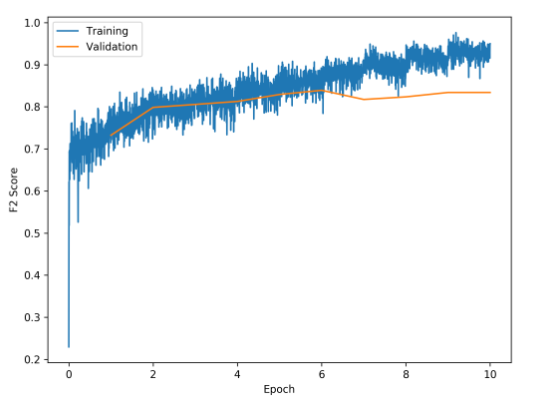
\includegraphics[width=\columnwidth]{AccuracyCurve.png}
    \caption{Accuracy (F2 score) for the training set and the validation set as a function of epoch. The training accuracy was plotted at the end of each batch of data, and the validation accuracy was plotted at the end of each epoch.}
\end{figure}

\begin{figure}
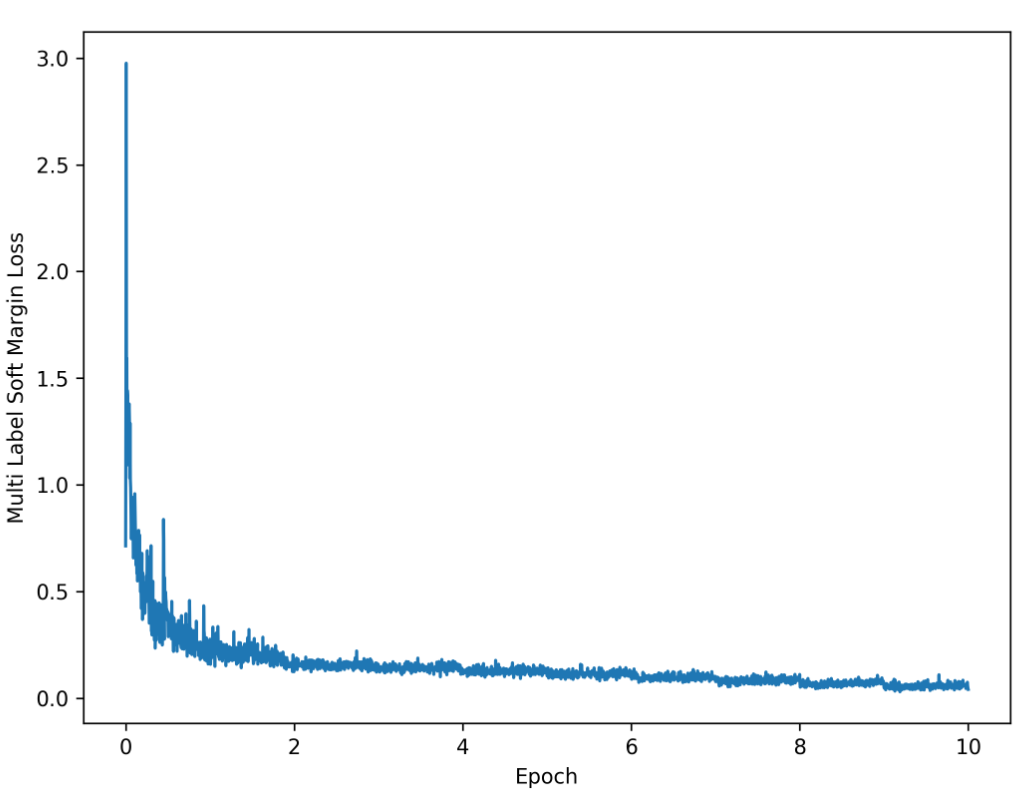
\includegraphics[width=\columnwidth]{LossCurve.png}
    \caption{Training loss (PyTorch multilabel soft margin loss) as a function of epoch. Even though we evaluate our model using F2 score, we use the multilabel soft margin loss function to train the model. The fact that a decrease in this loss corresponds to an increase in the training F2 score, plotted in Figure 1, shows that it is reasonable to use this as a loss function and evaluate our accuracy using the F2 score.}
\end{figure}


%------------------------------------------------------------------------
\section{Future Work}

Since the 6-layer CNN described above is starting to overfit the training data, we believe that that architecture will not be able to provide us with a validation accuracy much higher than the 0.83 that we have seen given the amount of training data that we have. We have two strategies to address this.

First, we will augment our data by training on each rotation and the mirror image of each rotation. These transformations will produce new, distinct images that have the exact same labels. This will effectively increase the amount of data we have to train on by a factor of eight. We expect that, given the new, larger, training set, we will be able to increase the complexity of this model (add more convolutional layers) and achieve a higher validation accuracy.

Second, we will implement a Res-Net design with many layers. Since this architecture performed very well in the ImageNet competition, we hope that it will be able to give a higher validation accuracy than the 6-layer VGG-Net-like CNN presented above. We will do a coarse hyperparameter optimization of each architecture, and we will fine tune the hyperparameters of our best-performing model.

One parameter that we have yet to tune is the cutoff for whether or not a label should be assigned to an image. Right now, the label is applied if the score is greater than 0.5, but this cutoff may not be optimal, especially for the rarer classes. We are considering ways to learn this parameter or at least do a better job setting it. The best Kaggle submissions so far have an F2 score of about 0.93, so, while we are pleased that we have already been able to get to within 0.1 of that, we are hoping that our future work will be able to close the gap.

%------------------------------------------------------------------------


{\small
\bibliographystyle{ieee}
\bibliography{references}
}

\end{document}
